
 

\chapter{Geometric Computation}
\label{sec:geom:algo}

In order to compute numerically the two-dimensional
integral~\eqref{lastexpression}, one must compute the area of the
intersection $\aire(A\,\cap\,(B-t))$ for different values of
$t\in\check{A}\oplus B$ (domain of integration) where $A$ and $B$ are
polygons. Note that $A$ and $B$ are not necessarily convex.
Computations of polygonal areas, intersections and Minkowski sums are
known problems in \emph{computational geometry}. The
textbook~\cite{ORourke:1998} is a rather nice introduction to that
topic. Most algorithms briefly described below are provided
there. Note that this chapter is only devoted to the computation of
the geometric features involved in the
integral~\eqref{lastexpression}. The problem of numerical integration
is treated in Chapter~\ref{sec:integrale}.

The intersection $A\,\cap\,(B-t)$ is a polygon. The computation of the
area of a polygon is straightforward, see
Section~\ref{sec:calcul:aire} for the case when the polygon is convex.

The computation of the intersection $A\,\cap\,(B-t)$ is easy when both
$A$ and $B$ are convex, see Section~\ref{sec:calcul:intersection}.
When either $A$ or $B$ is not convex, the intersection may be
complicated. In particular, it may not be connected.

The computation of the Minkowski sum $\check{A}\oplus B$ is rather
easy if $A$ or $B$ are convex, see Section~\ref{sec:calcul:somme}.

Hence the computation of the integral~\eqref{lastexpression} is easy
when both $A$ and $B$ are convex. This is why we propose to first
decompose $A$ and $B$ as unions of convex polygons:
\begin{equation}
  \label{eq:convex:decomp:A:B}
  A = \bigcup_{i=1}^n A_i,\qquad B = \bigcup_{j=1}^m B_j,
\end{equation}
where the areas of $A_{i}\cap A_{i'}$, respectively $B_{j}\cap
B_{j'}$, are equal to $0$ whenever $i\neq i'$, respectively $j\neq
j'$. An algorithm for computing such a decomposition is
described in Section~\ref{sec:decompo}. It is easy to check that the
integral~\eqref{lastexpression} can be written as:
\begin{equation}
  \label{eq:integral:decomposition}
  \int_{\check{A}\oplus B} \aire(A\,\cap\,(B-t)) \,\phi(t)
  \,dt =
  \sum_{i=1}^n \sum_{j=1}^m
  \int_{\check{A}_i\oplus B_j} \aire(A_i\,\cap\,(B_j-t)) \,\phi(t)
  \,dt.
\end{equation}
Based on the algorithm for decomposing polygons into convex ones and
tools for computing numerically the integral~\eqref{lastexpression}
for any pair $(A,B)$ of convex polygons (see Chapter
\ref{sec:integrale}), the integral~\eqref{lastexpression} for an
arbitrary pair of polygons can be computed using
Algorithm~\ref{algo:int:any:pair}.

% \begin{algorithm}
%   \caption{Integral computation for an arbitrary pair of polygons}
%   \label{algointanypair}
%   \begin{algorithmic}[1]
%     \REQUIRE Two polygons $A$ and $B$.
%     \ENSURE Computation of $\aire(A\,\cap\,(B-t))$ for an arbitrary vector 
%     $t$.
%     \STATE Compute convex polygons $A_1,\ldots,A_n$ such that
%     $A=\cup_{i=1}^n A_i$ and such that $\aire(A_{i}\cap A_{i'})=0$ if
%     $i\ne i'$.
%     \STATE Compute convex polygons $B_1,\ldots,B_m$ such that
%     $B=\cup_{j=1}^m B_j$ and such that $\aire(B_{j}\cap B_{j'})=0$ if
%     $j\ne j'$.
%     \STATE $\A=0$
%     \FORALL{$i=1,\ldots,n$}
%     \FORALL{$j=1,\ldots,m$}
%     \STATE Increment $\A$ by
%     $$\int_{\check{A}_i\oplus B_j} \aire(A_i\,\cap\,(B_j-t))\,
%     \phi(t)\,dt.$$ 
%     \ENDFOR
%     \ENDFOR
%   \end{algorithmic}
% \end{algorithm}

\begin{algorithm}
  \caption{Integral computation for an arbitrary pair of polygons}
  \label{algo:int:any:pair}
  \KwData{Two polygons $A$ and $B$, a dispersal function $\phi$.}
  \KwResult{Computation of $\aire(A\,\cap\,(B-t))$ for an arbitrary vector 
    $t$.}
  Compute convex polygons $A_1,\ldots,A_n$ such that
  $A=\bigcup_{i=1}^n A_i$ and such that $\aire(A_{i}\cap A_{i'})=0$ if
  $i\ne i'$\;
  Compute convex polygons $B_1,\ldots,B_m$ such that
  $B=\bigcup_{j=1}^m B_j$ and such that $\aire(B_{j}\cap B_{j'})=0$ if
  $j\ne j'$\;
  $\A=0$\;
  \For{$i=1,\ldots,n$}{
    \For{$j=1,\ldots,m$}{
      Increment $\A$ by
      $$\int_{\check{A}_i\oplus B_j} \aire(A_i\,\cap\,(B_j-t))\,
      \phi(t)\,dt;$$
    }
  }
\end{algorithm}

Below, convex polygons are represented as sequences of vertices
labeled counterclockwise:
\newline
$(v_0,\ldots,v_{n-1})$.
Many computations
involve cycling over vertices. Hence it is convenient
to use the convention $v_n=v_0$. All edges can be represented as
$e_i=(v_i,v_{i+1})$, $i=0,\ldots,n-1$.

% \section{Tester si un point est à l'intérieur d'un polygone}
% \label{sec:interieur}

% Un point est à
% l'intérieur d'un polygone convexe si et seulement si  ce point est toujours 
% à gauche lorsque l'on parcourt le périmètre du polygone.
% Voir Fig ~\ref{figinpoly}.
% \begin{figure}[htbp]
%   \begin{center}
%   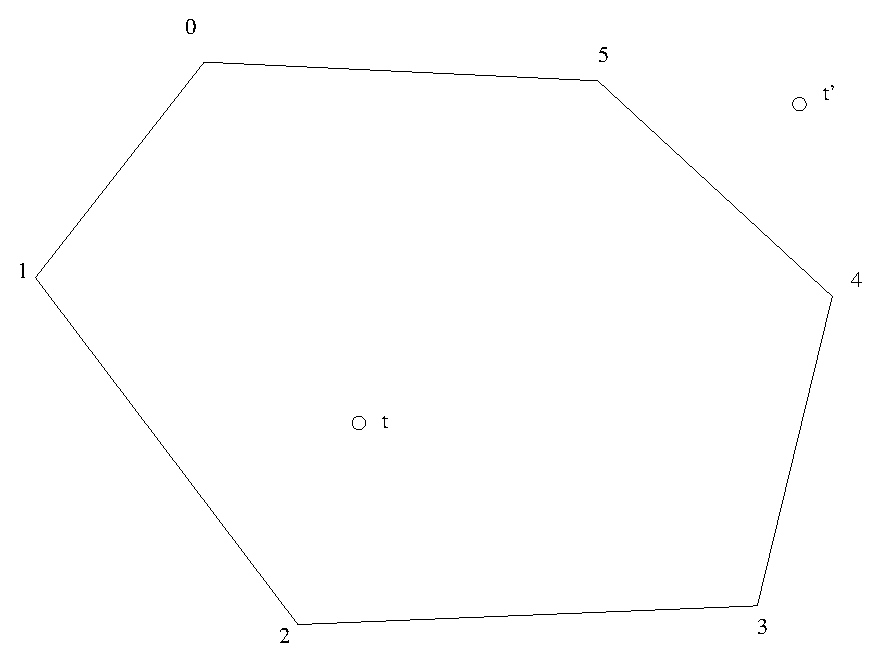
\includegraphics[width=9cm]{./graphics/inpoly.eps}
%   \end{center}
%   \caption{Tester si un point est à l'intérieur d'un polygone:
% le point $t'$ n'est pas à gauche de l'arête 4-5: il n'est donc pas dans
% le polygone, à l'inverse du point $t$ qui est à gauche de toutes les arêtes.}\label{figinpoly}
% \end{figure}

% \medskip
% {\small
% Remarque:
% Une méthode générale,  valide même
% pour un polygone non convexe, est basée sur le même principe.
% On calcule le nombre de points d'intersection d'une droite passant par
% le point avec le polygone. On peut prendre, par exemple, une droite
% horizontale. Si le nombre d'intersections à gauche du point testé est
% impair, le point est à l'intérieur.
% }

\section{Area of a convex polygon}
\label{sec:calcul:aire}

%% Remarques :
%% -----------
%%
%% - Il vaudrait mieux utiliser la formule générale. Pas tellement par
%%   souci d'efficacité, mais parce que le code serait plus clair.
%% - Les fonctions pour calculer des aires de triangles sont Area2
%%   (calcul sur des flottants) , Area2i (calcul sur des entiers). En
%%   fait, ces fonctions calculent le double de l'aire. En effet, ce
%%   résultat est entier si les coordonnées le sont aussi. Ce
%%   qui est assez bizarre, c'est que Area2i fait le calcul en
%%   flottants puis une conversion en entier. Ca permet d'avoir moins
%%   d'overflow. Mais il faut faire attention si Area2i n'est pas
%%   utilisé pour tester des prédicats (du genre C est à gauche de AB)
%%   car alors le résultat peut ne pas être correct.
%% - La fonction area_polygon_2 calcule le double de l'aire d'un
%%   polygone. Il faudrait changer le nom de l'argument et supprimer
%%   les sorties de débogage.

A convex polygon can be decomposed into triangles, see
Figure~\ref{figairepoly}. Thus its area is
the sum of its triangles areas. Each of them is computed using the
following formula
\begin{equation}
  \label{eq:triangle:area}
  \frac{1}{2}(x_B - x_A)(y_C - y_A) - (x_C - x_A)(y_B - y_A),
\end{equation}
where $A$, $B$ and $C$ are the triangle vertices and the $x$'s and
$y$'s are Cartesian coordinates. Equation~\eqref{eq:triangle:area}
yields a signed area. It is positive if $A$, $B$ and $C$ are ordered
counterclockwise, otherwise it is negative. The final result is exact
if the coordinates are integers.  The computing time depends on the
number of polygon vertices. Algorithm~\ref{algo:area} describes the
whole procedure. Note that if the polygon vertices are numbered
counterclockwise then the triangle vertices are also numbered
counterclockwise.
\begin{algorithm}[tbph]
  \caption{Area of a convex polygon. Triangle areas are computed
    using Equation~\eqref{eq:triangle:area}.}
  \label{algo:area}
  \KwData{Convex polygon with vertices (numbered counterclockwise)
    $v_0,\ldots,v_{n-1}$.}
  \KwResult{Area of the polygon.}
  $a=0$\;
  \For{$i=1,\ldots,n-2$}{
    $a=a+\aire(\text{triangle } v_{0},v_i,v_{i+1})$\;
  }
\end{algorithm}
%%
\begin{figure}[tbph]
  \begin{center}
    \includegraphics[width=9cm]{./VignetteDir/graphics/airepoly.eps}
    \caption{Decomposition of a convex polygon into triangles. An
      arbitrary vertex is connected to all non adjacent vertices.}
    \label{figairepoly}
  \end{center}
\end{figure}
%%

For area computation convexity is not an issue. The area of an
arbitrary polygon is also easy to compute. If
$(x_0,y_0),\ldots,(x_{n-1},y_{n-1})$ are the Cartesian coordinates of
the vertices (numbered counterclockwise) of a polygon, its area is
equal to
\begin{equation}
  \label{eq:area:any:polygon}
  \frac{1}{2}\sum_{i=1}^{n-1} (x_i+x_{i+1})(y_{i+1}-y_i).
\end{equation}

\section{Intersection of two convex polygons}
\label{sec:calcul:intersection}

%% Remarque : on peut avoir des problèmes numériques. Par exemple, on
%% peut tester a meets b positivement et avoir un pb avec le calcul de
%% l'intersection de a et b. Le test intersection de a et de b =
%% premier sommet du plygone résultat peut aussi être problématique (?).

Here we focus on the case when the boundaries of the two convex
polygons $P$ and $Q$ meet each other: the cases where the intersection
is void or where one polygon is included in the other one are not
considered.

The intersection $P\cap Q$ is a convex polygon whose vertices are
vertices of $P$ or vertices of $Q$ or intersection of edges of $P$
with edges of $Q$. The intersection can be computed using the
algorithm described in \cite[Section 7.6]{ORourke:1998}. Two orientated
edges $a\subset P$ and $b\subset Q$ are chosen. The edges $a$ and $b$
are advanced so  that all the vertices of $P\cap Q$
can be detected and recorded, see
Algorithm~\ref{algo:intersection:convex:poly}. Note that special cases
are not treated: the algorithm is valid if $P$ and $Q$ are in general
relative position, i.e.\ their boundaries cross only at the interior
of edges. Also the implementation of this algorithm requires some
further low-level functions:
\begin{itemize}
\item Test whether two segments meet.
\item Compute the intersection of two segments.
\item The advancing rule can be reformulated and requires only the
  computation of signed areas see \cite[Section 7.6]{ORourke:1998} for
  further details.
\end{itemize}

\begin{algorithm}[tbph]
  \caption{Intersection of two convex polygons}
  \label{algo:intersection:convex:poly}
  \KwData{Two convex polygons $P$ and $Q$}
  \KwResult{Computation of $P\,\cap\,Q$.}
  Choose an edge $a$ of $P$ and an edge $b$ of $Q$\;
  $R=\emptyset$\;
  \Repeat{both $a$ and $b$ cycle along $P$ and $Q$ boundaries}{
    \eIf{$a$ meets $b$}{
      \eIf{$a\cap b$ coincides with the first vertex of $R$}{
        Terminate\;
      }{
        Add $a\cap b$ to $R$\;
      }
      Advance either $a$ or $b$\;
    }{
      \eIf{One edge points toward the line containing the
        other}{
        Advance it\;
      }{
        \eIf{One edge is on the right-hand side of the other}{
          Advance it\;
        }{
          Advance either $a$ or $b$\;
        }
      }
    }
  }
\end{algorithm}

\section{Minkowski sum of convex polygons}
\label{sec:calcul:somme}

Let $P$ and $Q$ be two convex polygons. An algorithm for computing the
so-called convolution of $P$ and $Q$ is described in~\cite[Section
8.4]{ORourke:1998}. When both $P$ and $Q$ are convex, the convolution
is equivalent to the Minkowski sum. The computation of the convolution
is based on the \emph{star diagram} of $P$ and $Q$ edges. For any edge
$e$ of $P$ Let $\alpha(e)\in[0,2\pi)$ be the angle of $e$ with an
arbitrary axis. The star diagram is a polar representation of the
$\alpha's$. The Algorithm~\ref{algo:minkowski} shows how to compute
the Minkowski sum from the star diagram. Due to the convexity
assumption, $\alpha$ is increasing on the set of edges of a polygon if
the reference axis is parallel to its first edge.
\begin{algorithm}[tbph]
  \caption{Minkowski sum of two convex polygons.}
  \label{algo:minkowski}
  \KwData{Two convex polygons $P$ and $Q$.}
  \KwResult{The Minkowski sum $P\oplus Q$.}
  \tcp{Star diagram}
  Compute $\alpha$ for all edges of $P$ and $Q$ taking as the
  reference axis a line parallel to the first edge of $P$\;
  Sort the $\alpha$'s: $\alpha_k$, $k=0,\ldots,n+m-1$ where $n$ is the
  number of $P$-vertices and $m$ is the number of $Q$-vertices\;
  $R=\{\text{first vertex of }P\}$\;
  \For{$k=0,\ldots,n+m-1$}{
    Add to $R$ the latter vertex of $R$ translated by $\vec{e}$ where $e$ is
    the edge associated with $\alpha_k$\;
}
\end{algorithm}

\section{Convex partitioning of a polygon }
\label{sec:decompo}

In order to implement Algorithm~\ref{algo:int:any:pair}, one needs to
decompose an arbitrary polygon into convex polygons. The decomposition
algorithm is three-step:
\begin{enumerate}
\item The polygon $P$ is triangulated using an ear removal algorithm,
  see e.g.\ \cite[Section 1.6]{ORourke:1998}.
\item Essential diagonals of the triangulation are identified.
\item The convex subpolygons are created.
\end{enumerate}
An internal (resp.\ external) diagonal is a segment joining two
vertices which is contained in (resp.\ lies outside) the polygon. An
ear is a triangle inside the polygon whose vertices are three
consecutive vertices $a,b,c$ of the polygon, i.e. $ac$ is an internal
diagonal. 

The triangulation algorithm, see Algorithm~\ref{algo:triangulation},
consists in successive ear removals. In order to test whether a vertex
$v_i$ is an ear tip, one tests whether $v_{i-1}v_{i+1}$ is an internal
diagonal. The latter test is decomposed into two steps: first test
whether $v_{i-1}v_{i+1}$ is a diagonal (internal or external), second
test if $v_{i-1}v_{i+1}$ is internal. The first test involves edge
intersection tests (loop along the edges). For the second test, one
has to consider two cases:  $v_{i}$ is convex or reflex. The second
test requires only computation of signed areas.


The triangulation yields internal diagonals (inner edges of the
triangulation). 
A non-essential diagonal divides two adjacent cells
whose union is still convex. It is easy to check that a diagonal is
non-essential if both  its ends are convex. 



\begin{algorithm}[tbph]
  \caption{Triangulation of a polygon.}
  \label{algo:triangulation}
  \KwData{A polygon $P$ with vertices $v_0,\ldots,v_{n-1}$.}
  \KwResult{A triangulation of $P$}
  \tcp{Find ear tips}
  \For{$i=0,\ldots,n-1$}{
    \If{$v_{i-1}v_{i+1}$ is an internal diagonal}{
      Set $v_i$ as an ear tip\;
    }
  }
  $T=\emptyset$\;
  $v=$ first vertex of $P$\;
  \While{$P$ has more than $3$ vertices}{
    \If{$v$ is an ear tip}{
      Add to $T$ the triangle $uvw$ where $u$ is the vertex previous
      to $v$ and $w$ is the vertex next to $v$\;
      \tcp{Update ear tip status of $u$ and $w$}
      \If{the vertices before and after $u$ form a diagonal}{
        Set $u$ as an ear tip\;
      }
      \If{the vertices before and after $v$ form a diagonal}{
        Set $v$ as an ear tip\;
      }
      Remove $v$ from $P$\;
    }
    Advance $v$\;
  }
\end{algorithm}

The last step is to split the polygon according to computed essential
diagonals, see Algorithm~\ref{algo:split}.

\begin{algorithm}
  \caption{Creation of convex polygons from the essential diagonals}

  \label{algo:split}
\KwData{A nonconvex polygon: its $nvertices$ vertices and $ndiagonals$
diagonals; the essential diagonals are marked.
The sides of the polygon are essential diagonals.}
\KwResult{The $np$ convex subpolygons: their vertices are stored
  anticlockwise in $polyg$.}
$np=0$\\
\While{there is an essential diagonal}
{ $(v_a,v_b)$ = any  essential diagonal\\
$start = va$\\
\While{ $vb != start$}
{store $(v_a,v_b)$ into $polyg[np]$\\
mark $(v_a,v_b)$ non-essential\\
\tcp{Determine the following diagonal:}
$(v_b,v_c)$ is the diagonal starting from $v_b$ and such as the angle
$(v_a,v_b,v_c)$ is minimum\\
$v_a=v_b; v_b=v_c$
}
$np=np+1$
}
\end{algorithm}


